% Options for packages loaded elsewhere
\PassOptionsToPackage{unicode}{hyperref}
\PassOptionsToPackage{hyphens}{url}
%
\documentclass[
]{article}
\title{COVID-19 Vaccination Rate Mini Project}
\author{Ari\_Fon (PID: A15390446)}
\date{3/3/2022}

\usepackage{amsmath,amssymb}
\usepackage{lmodern}
\usepackage{iftex}
\ifPDFTeX
  \usepackage[T1]{fontenc}
  \usepackage[utf8]{inputenc}
  \usepackage{textcomp} % provide euro and other symbols
\else % if luatex or xetex
  \usepackage{unicode-math}
  \defaultfontfeatures{Scale=MatchLowercase}
  \defaultfontfeatures[\rmfamily]{Ligatures=TeX,Scale=1}
\fi
% Use upquote if available, for straight quotes in verbatim environments
\IfFileExists{upquote.sty}{\usepackage{upquote}}{}
\IfFileExists{microtype.sty}{% use microtype if available
  \usepackage[]{microtype}
  \UseMicrotypeSet[protrusion]{basicmath} % disable protrusion for tt fonts
}{}
\makeatletter
\@ifundefined{KOMAClassName}{% if non-KOMA class
  \IfFileExists{parskip.sty}{%
    \usepackage{parskip}
  }{% else
    \setlength{\parindent}{0pt}
    \setlength{\parskip}{6pt plus 2pt minus 1pt}}
}{% if KOMA class
  \KOMAoptions{parskip=half}}
\makeatother
\usepackage{xcolor}
\IfFileExists{xurl.sty}{\usepackage{xurl}}{} % add URL line breaks if available
\IfFileExists{bookmark.sty}{\usepackage{bookmark}}{\usepackage{hyperref}}
\hypersetup{
  pdftitle={COVID-19 Vaccination Rate Mini Project},
  pdfauthor={Ari\_Fon (PID: A15390446)},
  hidelinks,
  pdfcreator={LaTeX via pandoc}}
\urlstyle{same} % disable monospaced font for URLs
\usepackage[margin=1in]{geometry}
\usepackage{color}
\usepackage{fancyvrb}
\newcommand{\VerbBar}{|}
\newcommand{\VERB}{\Verb[commandchars=\\\{\}]}
\DefineVerbatimEnvironment{Highlighting}{Verbatim}{commandchars=\\\{\}}
% Add ',fontsize=\small' for more characters per line
\usepackage{framed}
\definecolor{shadecolor}{RGB}{248,248,248}
\newenvironment{Shaded}{\begin{snugshade}}{\end{snugshade}}
\newcommand{\AlertTok}[1]{\textcolor[rgb]{0.94,0.16,0.16}{#1}}
\newcommand{\AnnotationTok}[1]{\textcolor[rgb]{0.56,0.35,0.01}{\textbf{\textit{#1}}}}
\newcommand{\AttributeTok}[1]{\textcolor[rgb]{0.77,0.63,0.00}{#1}}
\newcommand{\BaseNTok}[1]{\textcolor[rgb]{0.00,0.00,0.81}{#1}}
\newcommand{\BuiltInTok}[1]{#1}
\newcommand{\CharTok}[1]{\textcolor[rgb]{0.31,0.60,0.02}{#1}}
\newcommand{\CommentTok}[1]{\textcolor[rgb]{0.56,0.35,0.01}{\textit{#1}}}
\newcommand{\CommentVarTok}[1]{\textcolor[rgb]{0.56,0.35,0.01}{\textbf{\textit{#1}}}}
\newcommand{\ConstantTok}[1]{\textcolor[rgb]{0.00,0.00,0.00}{#1}}
\newcommand{\ControlFlowTok}[1]{\textcolor[rgb]{0.13,0.29,0.53}{\textbf{#1}}}
\newcommand{\DataTypeTok}[1]{\textcolor[rgb]{0.13,0.29,0.53}{#1}}
\newcommand{\DecValTok}[1]{\textcolor[rgb]{0.00,0.00,0.81}{#1}}
\newcommand{\DocumentationTok}[1]{\textcolor[rgb]{0.56,0.35,0.01}{\textbf{\textit{#1}}}}
\newcommand{\ErrorTok}[1]{\textcolor[rgb]{0.64,0.00,0.00}{\textbf{#1}}}
\newcommand{\ExtensionTok}[1]{#1}
\newcommand{\FloatTok}[1]{\textcolor[rgb]{0.00,0.00,0.81}{#1}}
\newcommand{\FunctionTok}[1]{\textcolor[rgb]{0.00,0.00,0.00}{#1}}
\newcommand{\ImportTok}[1]{#1}
\newcommand{\InformationTok}[1]{\textcolor[rgb]{0.56,0.35,0.01}{\textbf{\textit{#1}}}}
\newcommand{\KeywordTok}[1]{\textcolor[rgb]{0.13,0.29,0.53}{\textbf{#1}}}
\newcommand{\NormalTok}[1]{#1}
\newcommand{\OperatorTok}[1]{\textcolor[rgb]{0.81,0.36,0.00}{\textbf{#1}}}
\newcommand{\OtherTok}[1]{\textcolor[rgb]{0.56,0.35,0.01}{#1}}
\newcommand{\PreprocessorTok}[1]{\textcolor[rgb]{0.56,0.35,0.01}{\textit{#1}}}
\newcommand{\RegionMarkerTok}[1]{#1}
\newcommand{\SpecialCharTok}[1]{\textcolor[rgb]{0.00,0.00,0.00}{#1}}
\newcommand{\SpecialStringTok}[1]{\textcolor[rgb]{0.31,0.60,0.02}{#1}}
\newcommand{\StringTok}[1]{\textcolor[rgb]{0.31,0.60,0.02}{#1}}
\newcommand{\VariableTok}[1]{\textcolor[rgb]{0.00,0.00,0.00}{#1}}
\newcommand{\VerbatimStringTok}[1]{\textcolor[rgb]{0.31,0.60,0.02}{#1}}
\newcommand{\WarningTok}[1]{\textcolor[rgb]{0.56,0.35,0.01}{\textbf{\textit{#1}}}}
\usepackage{longtable,booktabs,array}
\usepackage{calc} % for calculating minipage widths
% Correct order of tables after \paragraph or \subparagraph
\usepackage{etoolbox}
\makeatletter
\patchcmd\longtable{\par}{\if@noskipsec\mbox{}\fi\par}{}{}
\makeatother
% Allow footnotes in longtable head/foot
\IfFileExists{footnotehyper.sty}{\usepackage{footnotehyper}}{\usepackage{footnote}}
\makesavenoteenv{longtable}
\usepackage{graphicx}
\makeatletter
\def\maxwidth{\ifdim\Gin@nat@width>\linewidth\linewidth\else\Gin@nat@width\fi}
\def\maxheight{\ifdim\Gin@nat@height>\textheight\textheight\else\Gin@nat@height\fi}
\makeatother
% Scale images if necessary, so that they will not overflow the page
% margins by default, and it is still possible to overwrite the defaults
% using explicit options in \includegraphics[width, height, ...]{}
\setkeys{Gin}{width=\maxwidth,height=\maxheight,keepaspectratio}
% Set default figure placement to htbp
\makeatletter
\def\fps@figure{htbp}
\makeatother
\setlength{\emergencystretch}{3em} % prevent overfull lines
\providecommand{\tightlist}{%
  \setlength{\itemsep}{0pt}\setlength{\parskip}{0pt}}
\setcounter{secnumdepth}{-\maxdimen} % remove section numbering
\ifLuaTeX
  \usepackage{selnolig}  % disable illegal ligatures
\fi

\begin{document}
\maketitle

Here we downloaded the data from file called ``Statewide COVID-19
Vaccines Administered by ZIP Code'' using website
\url{https://data.ca.gov/dataset/covid-19-vaccine-progress-dashboard-data-by-zip-code}

\#First step is to import/read vaccination data

\begin{Shaded}
\begin{Highlighting}[]
\NormalTok{vax }\OtherTok{\textless{}{-}} \FunctionTok{read.csv}\NormalTok{(}\StringTok{"covid19vaccinesbyzipcode\_test.csv"}\NormalTok{)}
\FunctionTok{head}\NormalTok{(vax)}
\end{Highlighting}
\end{Shaded}

\begin{verbatim}
##   as_of_date zip_code_tabulation_area local_health_jurisdiction         county
## 1 2021-01-05                    92549                 Riverside      Riverside
## 2 2021-01-05                    92130                 San Diego      San Diego
## 3 2021-01-05                    92397            San Bernardino San Bernardino
## 4 2021-01-05                    94563              Contra Costa   Contra Costa
## 5 2021-01-05                    94519              Contra Costa   Contra Costa
## 6 2021-01-05                    91042               Los Angeles    Los Angeles
##   vaccine_equity_metric_quartile                 vem_source
## 1                              3 Healthy Places Index Score
## 2                              4 Healthy Places Index Score
## 3                              3 Healthy Places Index Score
## 4                              4 Healthy Places Index Score
## 5                              3 Healthy Places Index Score
## 6                              2 Healthy Places Index Score
##   age12_plus_population age5_plus_population persons_fully_vaccinated
## 1                2348.4                 2461                       NA
## 2               46300.3                53102                       61
## 3                3695.6                 4225                       NA
## 4               17216.1                18896                       NA
## 5               16861.2                18678                       NA
## 6               23962.2                25741                       NA
##   persons_partially_vaccinated percent_of_population_fully_vaccinated
## 1                           NA                                     NA
## 2                           27                               0.001149
## 3                           NA                                     NA
## 4                           NA                                     NA
## 5                           NA                                     NA
## 6                           NA                                     NA
##   percent_of_population_partially_vaccinated
## 1                                         NA
## 2                                   0.000508
## 3                                         NA
## 4                                         NA
## 5                                         NA
## 6                                         NA
##   percent_of_population_with_1_plus_dose booster_recip_count
## 1                                     NA                  NA
## 2                               0.001657                  NA
## 3                                     NA                  NA
## 4                                     NA                  NA
## 5                                     NA                  NA
## 6                                     NA                  NA
##                                                                redacted
## 1 Information redacted in accordance with CA state privacy requirements
## 2 Information redacted in accordance with CA state privacy requirements
## 3 Information redacted in accordance with CA state privacy requirements
## 4 Information redacted in accordance with CA state privacy requirements
## 5 Information redacted in accordance with CA state privacy requirements
## 6 Information redacted in accordance with CA state privacy requirements
\end{verbatim}

\begin{quote}
Q1. What column details the total number of people fully vaccinated?
\end{quote}

persons\_fully\_vaccinated

\begin{quote}
Q2. What column details the Zip code tabulation area?
\end{quote}

zip\_code\_tabulation\_area

\begin{quote}
Q3. What is the earliest date in this dataset?
\end{quote}

2021-01-05

\begin{quote}
Q4. What is the latest date in this dataset?
\end{quote}

2022-03-01

\begin{Shaded}
\begin{Highlighting}[]
\NormalTok{vax}\SpecialCharTok{$}\NormalTok{as\_of\_date[}\FunctionTok{nrow}\NormalTok{(vax)]}
\end{Highlighting}
\end{Shaded}

\begin{verbatim}
## [1] "2022-03-01"
\end{verbatim}

\begin{Shaded}
\begin{Highlighting}[]
\NormalTok{skimr}\SpecialCharTok{::}\FunctionTok{skim}\NormalTok{(vax)}
\end{Highlighting}
\end{Shaded}

\begin{longtable}[]{@{}ll@{}}
\caption{Data summary}\tabularnewline
\toprule
\endhead
Name & vax \\
Number of rows & 107604 \\
Number of columns & 15 \\
\_\_\_\_\_\_\_\_\_\_\_\_\_\_\_\_\_\_\_\_\_\_\_ & \\
Column type frequency: & \\
character & 5 \\
numeric & 10 \\
\_\_\_\_\_\_\_\_\_\_\_\_\_\_\_\_\_\_\_\_\_\_\_\_ & \\
Group variables & None \\
\bottomrule
\end{longtable}

\textbf{Variable type: character}

\begin{longtable}[]{@{}lrrrrrrr@{}}
\toprule
skim\_variable & n\_missing & complete\_rate & min & max & empty &
n\_unique & whitespace \\
\midrule
\endhead
as\_of\_date & 0 & 1 & 10 & 10 & 0 & 61 & 0 \\
local\_health\_jurisdiction & 0 & 1 & 0 & 15 & 305 & 62 & 0 \\
county & 0 & 1 & 0 & 15 & 305 & 59 & 0 \\
vem\_source & 0 & 1 & 15 & 26 & 0 & 3 & 0 \\
redacted & 0 & 1 & 2 & 69 & 0 & 2 & 0 \\
\bottomrule
\end{longtable}

\textbf{Variable type: numeric}

\begin{longtable}[]{@{}
  >{\raggedright\arraybackslash}p{(\columnwidth - 20\tabcolsep) * \real{0.32}}
  >{\raggedleft\arraybackslash}p{(\columnwidth - 20\tabcolsep) * \real{0.08}}
  >{\raggedleft\arraybackslash}p{(\columnwidth - 20\tabcolsep) * \real{0.11}}
  >{\raggedleft\arraybackslash}p{(\columnwidth - 20\tabcolsep) * \real{0.07}}
  >{\raggedleft\arraybackslash}p{(\columnwidth - 20\tabcolsep) * \real{0.07}}
  >{\raggedleft\arraybackslash}p{(\columnwidth - 20\tabcolsep) * \real{0.05}}
  >{\raggedleft\arraybackslash}p{(\columnwidth - 20\tabcolsep) * \real{0.07}}
  >{\raggedleft\arraybackslash}p{(\columnwidth - 20\tabcolsep) * \real{0.07}}
  >{\raggedleft\arraybackslash}p{(\columnwidth - 20\tabcolsep) * \real{0.07}}
  >{\raggedleft\arraybackslash}p{(\columnwidth - 20\tabcolsep) * \real{0.07}}
  >{\raggedright\arraybackslash}p{(\columnwidth - 20\tabcolsep) * \real{0.05}}@{}}
\toprule
\begin{minipage}[b]{\linewidth}\raggedright
skim\_variable
\end{minipage} & \begin{minipage}[b]{\linewidth}\raggedleft
n\_missing
\end{minipage} & \begin{minipage}[b]{\linewidth}\raggedleft
complete\_rate
\end{minipage} & \begin{minipage}[b]{\linewidth}\raggedleft
mean
\end{minipage} & \begin{minipage}[b]{\linewidth}\raggedleft
sd
\end{minipage} & \begin{minipage}[b]{\linewidth}\raggedleft
p0
\end{minipage} & \begin{minipage}[b]{\linewidth}\raggedleft
p25
\end{minipage} & \begin{minipage}[b]{\linewidth}\raggedleft
p50
\end{minipage} & \begin{minipage}[b]{\linewidth}\raggedleft
p75
\end{minipage} & \begin{minipage}[b]{\linewidth}\raggedleft
p100
\end{minipage} & \begin{minipage}[b]{\linewidth}\raggedright
hist
\end{minipage} \\
\midrule
\endhead
zip\_code\_tabulation\_area & 0 & 1.00 & 93665.11 & 1817.39 & 90001 &
92257.75 & 93658.50 & 95380.50 & 97635.0 & ▃▅▅▇▁ \\
vaccine\_equity\_metric\_quartile & 5307 & 0.95 & 2.44 & 1.11 & 1 & 1.00
& 2.00 & 3.00 & 4.0 & ▇▇▁▇▇ \\
age12\_plus\_population & 0 & 1.00 & 18895.04 & 18993.91 & 0 & 1346.95 &
13685.10 & 31756.12 & 88556.7 & ▇▃▂▁▁ \\
age5\_plus\_population & 0 & 1.00 & 20875.24 & 21106.02 & 0 & 1460.50 &
15364.00 & 34877.00 & 101902.0 & ▇▃▂▁▁ \\
persons\_fully\_vaccinated & 18338 & 0.83 & 12155.61 & 13063.88 & 11 &
1066.25 & 7374.50 & 20005.00 & 77744.0 & ▇▃▁▁▁ \\
persons\_partially\_vaccinated & 18338 & 0.83 & 831.74 & 1348.68 & 11 &
76.00 & 372.00 & 1076.00 & 34219.0 & ▇▁▁▁▁ \\
percent\_of\_population\_fully\_vaccinated & 18338 & 0.83 & 0.51 & 0.26
& 0 & 0.33 & 0.54 & 0.70 & 1.0 & ▅▅▇▇▃ \\
percent\_of\_population\_partially\_vaccinated & 18338 & 0.83 & 0.05 &
0.09 & 0 & 0.01 & 0.03 & 0.05 & 1.0 & ▇▁▁▁▁ \\
percent\_of\_population\_with\_1\_plus\_dose & 18338 & 0.83 & 0.54 &
0.28 & 0 & 0.36 & 0.58 & 0.75 & 1.0 & ▅▃▆▇▅ \\
booster\_recip\_count & 64317 & 0.40 & 4100.55 & 5900.21 & 11 & 176.00 &
1136.00 & 6154.50 & 50602.0 & ▇▁▁▁▁ \\
\bottomrule
\end{longtable}

\begin{quote}
Q5. How many numeric columns are in this dataset?
\end{quote}

9

\begin{quote}
Q6. Note that there are ``missing values'' in the dataset. How many NA
values there in the persons\_fully\_vaccinated column?
\end{quote}

18338

\begin{quote}
Q7. What percent of persons\_fully\_vaccinated values are missing (to 2
significant figures)?
\end{quote}

\begin{Shaded}
\begin{Highlighting}[]
\FunctionTok{round}\NormalTok{((}\DecValTok{18338}\SpecialCharTok{/}\DecValTok{107604}\NormalTok{)}\SpecialCharTok{*}\DecValTok{100}\NormalTok{, }\DecValTok{2}\NormalTok{)}
\end{Highlighting}
\end{Shaded}

\begin{verbatim}
## [1] 17.04
\end{verbatim}

\begin{quote}
Q8. {[}Optional{]}: Why might this data be missing?
\end{quote}

Not everyone gets them from the CDC, such as people who get them
somewhere else such as the VA or elsewhere.

\#Working with Dates

\begin{Shaded}
\begin{Highlighting}[]
\FunctionTok{library}\NormalTok{(lubridate)}
\end{Highlighting}
\end{Shaded}

\begin{verbatim}
## 
## Attaching package: 'lubridate'
\end{verbatim}

\begin{verbatim}
## The following objects are masked from 'package:base':
## 
##     date, intersect, setdiff, union
\end{verbatim}

\begin{Shaded}
\begin{Highlighting}[]
\FunctionTok{today}\NormalTok{()}
\end{Highlighting}
\end{Shaded}

\begin{verbatim}
## [1] "2022-03-03"
\end{verbatim}

\begin{Shaded}
\begin{Highlighting}[]
\CommentTok{\# Specify that we are using the year{-}month{-}day format}
\NormalTok{vax}\SpecialCharTok{$}\NormalTok{as\_of\_date }\OtherTok{\textless{}{-}} \FunctionTok{ymd}\NormalTok{(vax}\SpecialCharTok{$}\NormalTok{as\_of\_date)}
\end{Highlighting}
\end{Shaded}

\begin{Shaded}
\begin{Highlighting}[]
\FunctionTok{today}\NormalTok{() }\SpecialCharTok{{-}}\NormalTok{ vax}\SpecialCharTok{$}\NormalTok{as\_of\_date[}\DecValTok{1}\NormalTok{]}
\end{Highlighting}
\end{Shaded}

\begin{verbatim}
## Time difference of 422 days
\end{verbatim}

\begin{Shaded}
\begin{Highlighting}[]
\NormalTok{vax}\SpecialCharTok{$}\NormalTok{as\_of\_date[}\FunctionTok{nrow}\NormalTok{(vax)] }\SpecialCharTok{{-}}\NormalTok{ vax}\SpecialCharTok{$}\NormalTok{as\_of\_date[}\DecValTok{1}\NormalTok{]}
\end{Highlighting}
\end{Shaded}

\begin{verbatim}
## Time difference of 420 days
\end{verbatim}

\begin{Shaded}
\begin{Highlighting}[]
\NormalTok{age }\OtherTok{\textless{}{-}}\FunctionTok{today}\NormalTok{()}\SpecialCharTok{{-}}\FunctionTok{ymd}\NormalTok{(}\StringTok{"2000{-}01{-}20"}\NormalTok{)}
\NormalTok{age}
\end{Highlighting}
\end{Shaded}

\begin{verbatim}
## Time difference of 8078 days
\end{verbatim}

\begin{Shaded}
\begin{Highlighting}[]
\FunctionTok{time\_length}\NormalTok{(age, }\StringTok{"year"}\NormalTok{)}
\end{Highlighting}
\end{Shaded}

\begin{verbatim}
## [1] 22.11636
\end{verbatim}

\begin{quote}
Q9. How many days have passed since the last update of the dataset?
\end{quote}

time difference of 2 days

\begin{Shaded}
\begin{Highlighting}[]
\FunctionTok{today}\NormalTok{()}\SpecialCharTok{{-}}\NormalTok{vax}\SpecialCharTok{$}\NormalTok{as\_of\_date[}\FunctionTok{nrow}\NormalTok{(vax)]}
\end{Highlighting}
\end{Shaded}

\begin{verbatim}
## Time difference of 2 days
\end{verbatim}

\begin{quote}
Q10. How many unique dates are in the dataset (i.e.~how many different
dates are detailed)?
\end{quote}

61 unique dates in the dataset

\begin{Shaded}
\begin{Highlighting}[]
\NormalTok{udates }\OtherTok{\textless{}{-}} \FunctionTok{unique}\NormalTok{(vax}\SpecialCharTok{$}\NormalTok{as\_of\_date)}
\FunctionTok{length}\NormalTok{(udates)}
\end{Highlighting}
\end{Shaded}

\begin{verbatim}
## [1] 61
\end{verbatim}

\#Working with Zipcodes

\begin{Shaded}
\begin{Highlighting}[]
\FunctionTok{library}\NormalTok{(zipcodeR)}
\end{Highlighting}
\end{Shaded}

\begin{Shaded}
\begin{Highlighting}[]
\FunctionTok{geocode\_zip}\NormalTok{(}\StringTok{\textquotesingle{}92037\textquotesingle{}}\NormalTok{)}
\end{Highlighting}
\end{Shaded}

\begin{verbatim}
## # A tibble: 1 x 3
##   zipcode   lat   lng
##   <chr>   <dbl> <dbl>
## 1 92037    32.8 -117.
\end{verbatim}

\begin{Shaded}
\begin{Highlighting}[]
\FunctionTok{zip\_distance}\NormalTok{(}\StringTok{\textquotesingle{}92037\textquotesingle{}}\NormalTok{,}\StringTok{\textquotesingle{}92109\textquotesingle{}}\NormalTok{)}
\end{Highlighting}
\end{Shaded}

\begin{verbatim}
##   zipcode_a zipcode_b distance
## 1     92037     92109     2.33
\end{verbatim}

\begin{Shaded}
\begin{Highlighting}[]
\FunctionTok{reverse\_zipcode}\NormalTok{(}\FunctionTok{c}\NormalTok{(}\StringTok{\textquotesingle{}92037\textquotesingle{}}\NormalTok{, }\StringTok{"92109"}\NormalTok{) )}
\end{Highlighting}
\end{Shaded}

\begin{verbatim}
## # A tibble: 2 x 24
##   zipcode zipcode_type major_city post_office_city common_city_list county state
##   <chr>   <chr>        <chr>      <chr>                      <blob> <chr>  <chr>
## 1 92037   Standard     La Jolla   La Jolla, CA           <raw 20 B> San D~ CA   
## 2 92109   Standard     San Diego  San Diego, CA          <raw 21 B> San D~ CA   
## # ... with 17 more variables: lat <dbl>, lng <dbl>, timezone <chr>,
## #   radius_in_miles <dbl>, area_code_list <blob>, population <int>,
## #   population_density <dbl>, land_area_in_sqmi <dbl>,
## #   water_area_in_sqmi <dbl>, housing_units <int>,
## #   occupied_housing_units <int>, median_home_value <int>,
## #   median_household_income <int>, bounds_west <dbl>, bounds_east <dbl>,
## #   bounds_north <dbl>, bounds_south <dbl>
\end{verbatim}

\begin{Shaded}
\begin{Highlighting}[]
\CommentTok{\# Pull data for all ZIP codes in the dataset}
\NormalTok{zipdata }\OtherTok{\textless{}{-}} \FunctionTok{reverse\_zipcode}\NormalTok{(vax}\SpecialCharTok{$}\NormalTok{zip\_code\_tabulation\_area )}
\FunctionTok{head}\NormalTok{(zipdata)}
\end{Highlighting}
\end{Shaded}

\begin{verbatim}
## # A tibble: 6 x 24
##   zipcode zipcode_type major_city post_office_city common_city_list county state
##   <chr>   <chr>        <chr>      <chr>                      <blob> <chr>  <chr>
## 1 90001   Standard     Los Angel~ Los Angeles, CA        <raw 44 B> Los A~ CA   
## 2 90002   Standard     Los Angel~ Los Angeles, CA        <raw 47 B> Los A~ CA   
## 3 90003   Standard     Los Angel~ Los Angeles, CA        <raw 23 B> Los A~ CA   
## 4 90004   Standard     Los Angel~ Los Angeles, CA        <raw 34 B> Los A~ CA   
## 5 90005   Standard     Los Angel~ Los Angeles, CA        <raw 34 B> Los A~ CA   
## 6 90006   Standard     Los Angel~ Los Angeles, CA        <raw 23 B> Los A~ CA   
## # ... with 17 more variables: lat <dbl>, lng <dbl>, timezone <chr>,
## #   radius_in_miles <dbl>, area_code_list <blob>, population <int>,
## #   population_density <dbl>, land_area_in_sqmi <dbl>,
## #   water_area_in_sqmi <dbl>, housing_units <int>,
## #   occupied_housing_units <int>, median_home_value <int>,
## #   median_household_income <int>, bounds_west <dbl>, bounds_east <dbl>,
## #   bounds_north <dbl>, bounds_south <dbl>
\end{verbatim}

\#\#Focus on the San Diego area

Let's now focus in on the San Diego County area by restricting ourselves
first to vax\$county == ``San Diego'' entries. We have two main choices
on how to do this. The first using base R the second using the dplyr
package:

\begin{Shaded}
\begin{Highlighting}[]
\FunctionTok{library}\NormalTok{(dplyr)}
\end{Highlighting}
\end{Shaded}

\begin{verbatim}
## 
## Attaching package: 'dplyr'
\end{verbatim}

\begin{verbatim}
## The following objects are masked from 'package:stats':
## 
##     filter, lag
\end{verbatim}

\begin{verbatim}
## The following objects are masked from 'package:base':
## 
##     intersect, setdiff, setequal, union
\end{verbatim}

\begin{Shaded}
\begin{Highlighting}[]
\NormalTok{sd }\OtherTok{\textless{}{-}} \FunctionTok{filter}\NormalTok{(vax, county }\SpecialCharTok{==} \StringTok{"San Diego"}\NormalTok{)}
\FunctionTok{nrow}\NormalTok{(sd)}
\end{Highlighting}
\end{Shaded}

\begin{verbatim}
## [1] 6527
\end{verbatim}

\begin{Shaded}
\begin{Highlighting}[]
\NormalTok{sd}\FloatTok{.10} \OtherTok{\textless{}{-}} \FunctionTok{filter}\NormalTok{(vax, county }\SpecialCharTok{==} \StringTok{"San Diego"} \SpecialCharTok{\&}
\NormalTok{                age5\_plus\_population }\SpecialCharTok{\textgreater{}} \DecValTok{10000}\NormalTok{)}
\end{Highlighting}
\end{Shaded}

\begin{quote}
Q11. How many distinct zip codes are listed for San Diego County?
\end{quote}

107 distinct zip codes listed for SD county

\begin{Shaded}
\begin{Highlighting}[]
\NormalTok{uzip }\OtherTok{\textless{}{-}} \FunctionTok{unique}\NormalTok{(sd}\SpecialCharTok{$}\NormalTok{zip\_code\_tabulation\_area)}
\FunctionTok{length}\NormalTok{(uzip)}
\end{Highlighting}
\end{Shaded}

\begin{verbatim}
## [1] 107
\end{verbatim}

\begin{quote}
Q12. What San Diego County Zip code area has the largest 12 + Population
in this dataset?
\end{quote}

92154

\begin{Shaded}
\begin{Highlighting}[]
\NormalTok{sdmax12 }\OtherTok{\textless{}{-}} \FunctionTok{which.max}\NormalTok{(sd}\SpecialCharTok{$}\NormalTok{age12\_plus\_population)}
\FunctionTok{print}\NormalTok{(sdmax12)}
\end{Highlighting}
\end{Shaded}

\begin{verbatim}
## [1] 91
\end{verbatim}

\begin{Shaded}
\begin{Highlighting}[]
\NormalTok{sd}\SpecialCharTok{$}\NormalTok{zip\_code\_tabulation\_area[sdmax12]}
\end{Highlighting}
\end{Shaded}

\begin{verbatim}
## [1] 92154
\end{verbatim}

Using dplyr select all San Diego ``county'' entries on ``as\_of\_date''
``2022-02-22'' and use this for the following questions.

\begin{Shaded}
\begin{Highlighting}[]
\NormalTok{sd}\SpecialCharTok{$}\NormalTok{as\_of\_date[}\FunctionTok{nrow}\NormalTok{(sd)]}
\end{Highlighting}
\end{Shaded}

\begin{verbatim}
## [1] "2022-03-01"
\end{verbatim}

Let's do this with the most recent date in the data-set (2022-03-01).

\begin{quote}
Q13. What is the overall average ``Percent of Population Fully
Vaccinated'' value for all San Diego ``County'' as of ``2022-03-01''?
\end{quote}

\begin{Shaded}
\begin{Highlighting}[]
\CommentTok{\#filter to the day}
\NormalTok{sd.latest }\OtherTok{\textless{}{-}} \FunctionTok{filter}\NormalTok{(sd, as\_of\_date }\SpecialCharTok{==} \StringTok{"2022{-}03{-}01"}\NormalTok{)}
\FunctionTok{round}\NormalTok{(}\FunctionTok{mean}\NormalTok{(sd.latest}\SpecialCharTok{$}\NormalTok{percent\_of\_population\_fully\_vaccinated, }\AttributeTok{na.rm =} \ConstantTok{TRUE}\NormalTok{),}\DecValTok{2}\NormalTok{)}
\end{Highlighting}
\end{Shaded}

\begin{verbatim}
## [1] 0.71
\end{verbatim}

\begin{Shaded}
\begin{Highlighting}[]
\FunctionTok{summary}\NormalTok{(sd.latest}\SpecialCharTok{$}\NormalTok{percent\_of\_population\_fully\_vaccinated)}
\end{Highlighting}
\end{Shaded}

\begin{verbatim}
##    Min. 1st Qu.  Median    Mean 3rd Qu.    Max.    NA's 
## 0.01017 0.65132 0.72452 0.70529 0.82567 1.00000       1
\end{verbatim}

71\% overall average

\begin{quote}
Q14. Using either ggplot or base R graphics make a summary figure that
shows the distribution of Percent of Population Fully Vaccinated values
as of ``2022-03-01''?
\end{quote}

\begin{Shaded}
\begin{Highlighting}[]
\FunctionTok{hist}\NormalTok{(sd.latest}\SpecialCharTok{$}\NormalTok{percent\_of\_population\_fully\_vaccinated, }\AttributeTok{breaks =}\DecValTok{30}\NormalTok{)}
\end{Highlighting}
\end{Shaded}

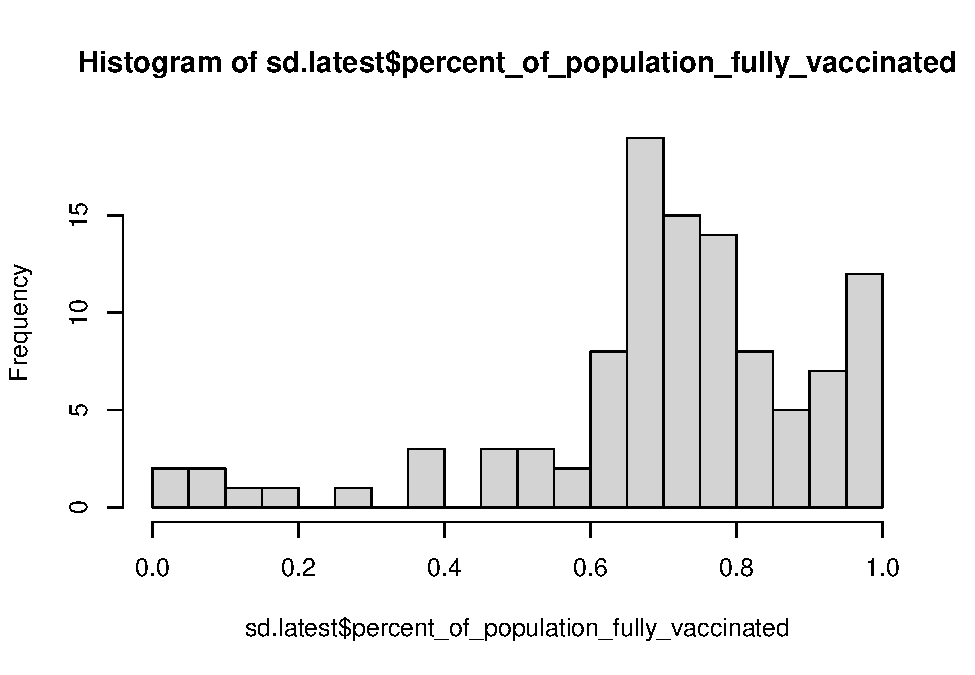
\includegraphics{COVID-19-Vax-mini-project_files/figure-latex/unnamed-chunk-26-1.pdf}

\begin{Shaded}
\begin{Highlighting}[]
\FunctionTok{library}\NormalTok{(ggplot2)}

\FunctionTok{ggplot}\NormalTok{(sd.latest) }\SpecialCharTok{+}\FunctionTok{aes}\NormalTok{(percent\_of\_population\_fully\_vaccinated)}\SpecialCharTok{+} \FunctionTok{geom\_histogram}\NormalTok{()}
\end{Highlighting}
\end{Shaded}

\begin{verbatim}
## `stat_bin()` using `bins = 30`. Pick better value with `binwidth`.
\end{verbatim}

\begin{verbatim}
## Warning: Removed 1 rows containing non-finite values (stat_bin).
\end{verbatim}

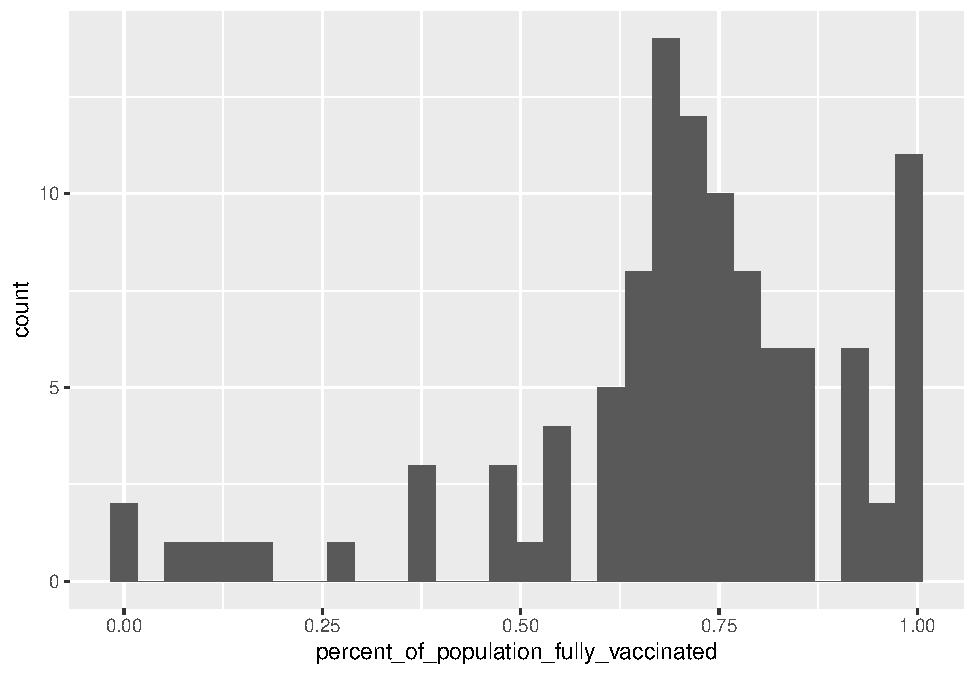
\includegraphics{COVID-19-Vax-mini-project_files/figure-latex/unnamed-chunk-27-1.pdf}

\hypertarget{focus-on-ucsdla-jolla}{%
\subsection{Focus on UCSD/La Jolla}\label{focus-on-ucsdla-jolla}}

\begin{Shaded}
\begin{Highlighting}[]
\NormalTok{ucsd }\OtherTok{\textless{}{-}} \FunctionTok{filter}\NormalTok{(sd, zip\_code\_tabulation\_area}\SpecialCharTok{==}\StringTok{"92037"}\NormalTok{)}
\NormalTok{ucsd[}\DecValTok{1}\NormalTok{,]}\SpecialCharTok{$}\NormalTok{age5\_plus\_population}
\end{Highlighting}
\end{Shaded}

\begin{verbatim}
## [1] 36144
\end{verbatim}

\begin{quote}
Q15. Using ggplot make a graph of the vaccination rate time course for
the 92037 ZIP code area:
\end{quote}

\begin{Shaded}
\begin{Highlighting}[]
\NormalTok{baseplot }\OtherTok{\textless{}{-}} \FunctionTok{ggplot}\NormalTok{(ucsd) }\SpecialCharTok{+}
  \FunctionTok{aes}\NormalTok{(as\_of\_date,}
\NormalTok{      percent\_of\_population\_fully\_vaccinated) }\SpecialCharTok{+}
  \FunctionTok{geom\_point}\NormalTok{() }\SpecialCharTok{+}
  \FunctionTok{geom\_line}\NormalTok{(}\AttributeTok{group=}\DecValTok{1}\NormalTok{) }\SpecialCharTok{+}
  \FunctionTok{ylim}\NormalTok{(}\FunctionTok{c}\NormalTok{(}\DecValTok{0}\NormalTok{,}\DecValTok{1}\NormalTok{)) }\SpecialCharTok{+}
  \FunctionTok{labs}\NormalTok{(}\AttributeTok{x=} \StringTok{"Date"}\NormalTok{, }\AttributeTok{y=}\StringTok{"Percent Vaccinated"}\NormalTok{, }\AttributeTok{title=} \StringTok{"Vaccination rate for La Jolla 92037"}\NormalTok{ )}
\NormalTok{baseplot}
\end{Highlighting}
\end{Shaded}

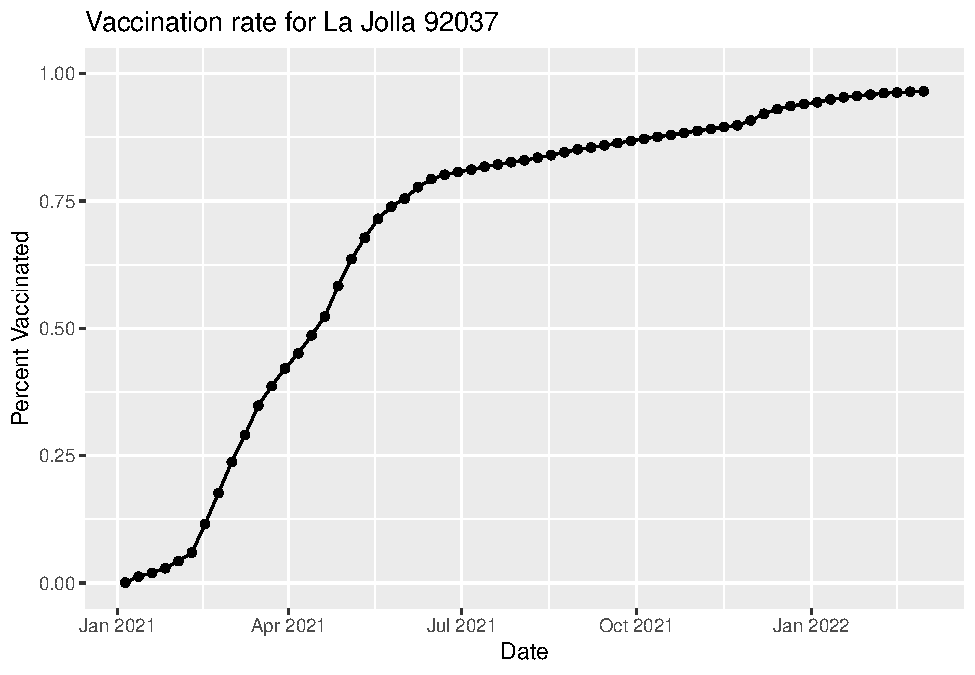
\includegraphics{COVID-19-Vax-mini-project_files/figure-latex/unnamed-chunk-29-1.pdf}

\#Comparing to similar sized areas

\begin{quote}
Q16. Calculate the mean ``Percent of Population Fully Vaccinated'' for
ZIP code areas with a population as large as 92037 (La Jolla)
as\_of\_date ``2022-02-22''. Add this as a straight horizontal line to
your plot from above with the geom\_hline() function?
\end{quote}

Add a line showing the average vaccination rate for all zip code areas
with a population jyst as large as 92037

\begin{Shaded}
\begin{Highlighting}[]
\NormalTok{baseplot }\SpecialCharTok{+} \FunctionTok{labs}\NormalTok{(}\AttributeTok{title=} \StringTok{"Vaccination rate for CA 92037 (UCSD)"}\NormalTok{)}
\end{Highlighting}
\end{Shaded}

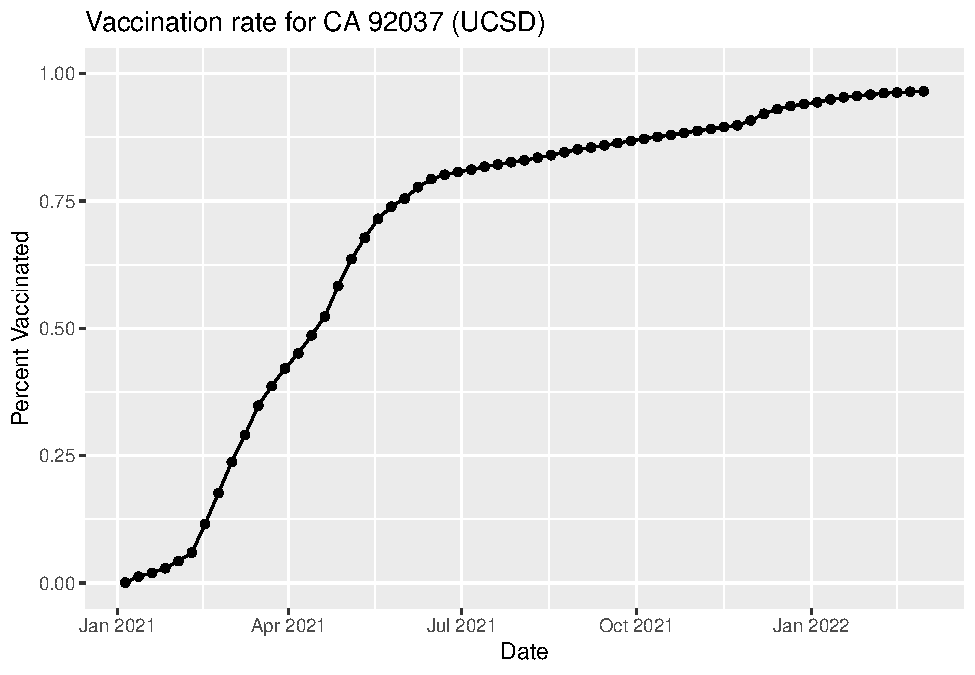
\includegraphics{COVID-19-Vax-mini-project_files/figure-latex/unnamed-chunk-30-1.pdf}
Add a line showing the average vaccination rate for all zip code areas
with a population jyst as large as 92037

\begin{Shaded}
\begin{Highlighting}[]
\CommentTok{\# Subset to all CA areas with a population as large as 92037}
\NormalTok{vax}\FloatTok{.36} \OtherTok{\textless{}{-}} \FunctionTok{filter}\NormalTok{(vax, age5\_plus\_population }\SpecialCharTok{\textgreater{}} \DecValTok{36144} \SpecialCharTok{\&}
\NormalTok{                as\_of\_date }\SpecialCharTok{==} \StringTok{"2022{-}03{-}01"}\NormalTok{)}

\FunctionTok{head}\NormalTok{(vax}\FloatTok{.36}\NormalTok{)}
\end{Highlighting}
\end{Shaded}

\begin{verbatim}
##   as_of_date zip_code_tabulation_area local_health_jurisdiction      county
## 1 2022-03-01                    95628                Sacramento  Sacramento
## 2 2022-03-01                    90808                Long Beach Los Angeles
## 3 2022-03-01                    92507                 Riverside   Riverside
## 4 2022-03-01                    92626                    Orange      Orange
## 5 2022-03-01                    93257                    Tulare      Tulare
## 6 2022-03-01                    90011               Los Angeles Los Angeles
##   vaccine_equity_metric_quartile                 vem_source
## 1                              3 Healthy Places Index Score
## 2                              4 Healthy Places Index Score
## 3                              1 Healthy Places Index Score
## 4                              3 Healthy Places Index Score
## 5                              1 Healthy Places Index Score
## 6                              1 Healthy Places Index Score
##   age12_plus_population age5_plus_population persons_fully_vaccinated
## 1               35579.0                38694                    28842
## 2               33952.3                37179                    29383
## 3               51432.5                55253                    34455
## 4               44238.8                47883                    33767
## 5               61519.8                70784                    42919
## 6               87902.8               101902                    65342
##   persons_partially_vaccinated percent_of_population_fully_vaccinated
## 1                         1990                               0.745387
## 2                         2112                               0.790312
## 3                         3947                               0.623586
## 4                         2937                               0.705198
## 5                         5868                               0.606338
## 6                        15255                               0.641224
##   percent_of_population_partially_vaccinated
## 1                                   0.051429
## 2                                   0.056806
## 3                                   0.071435
## 4                                   0.061337
## 5                                   0.082900
## 6                                   0.149703
##   percent_of_population_with_1_plus_dose booster_recip_count redacted
## 1                               0.796816               16913       No
## 2                               0.847118               17253       No
## 3                               0.695021               15073       No
## 4                               0.766535               17595       No
## 5                               0.689238               17740       No
## 6                               0.790927               19928       No
\end{verbatim}

\begin{Shaded}
\begin{Highlighting}[]
\NormalTok{ave}\FloatTok{.36} \OtherTok{\textless{}{-}} \FunctionTok{mean}\NormalTok{(vax}\FloatTok{.36}\SpecialCharTok{$}\NormalTok{percent\_of\_population\_fully\_vaccinated, }\AttributeTok{na.rm =} \ConstantTok{TRUE}\NormalTok{)}
\NormalTok{ave}\FloatTok{.36}
\end{Highlighting}
\end{Shaded}

\begin{verbatim}
## [1] 0.7353974
\end{verbatim}

\begin{Shaded}
\begin{Highlighting}[]
\NormalTok{baseplot }\SpecialCharTok{+} \FunctionTok{labs}\NormalTok{(}\AttributeTok{title=} \StringTok{"Vaccination rate for CA 92037 (UCSD)"}\NormalTok{) }\SpecialCharTok{+} \FunctionTok{geom\_hline}\NormalTok{(}\AttributeTok{yintercept=}\NormalTok{ave}\FloatTok{.36}\NormalTok{, }\AttributeTok{linetype=} \StringTok{"dashed"}\NormalTok{, }\AttributeTok{col=}\StringTok{"red"}\NormalTok{)}
\end{Highlighting}
\end{Shaded}

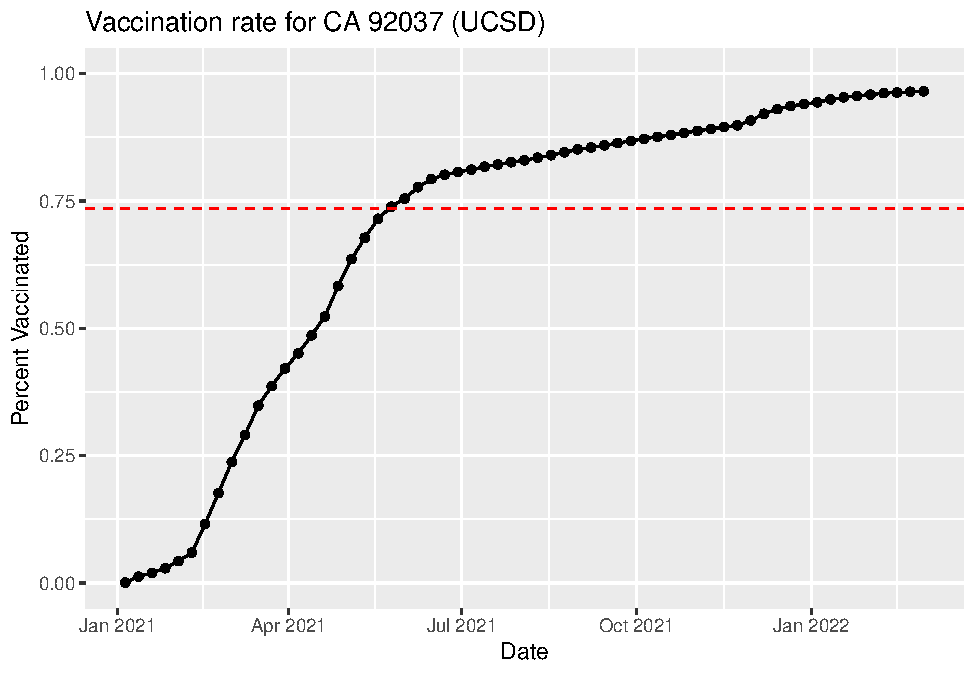
\includegraphics{COVID-19-Vax-mini-project_files/figure-latex/unnamed-chunk-32-1.pdf}

\begin{quote}
Q17. What is the 6 number summary (Min, 1st Qu., Median, Mean, 3rd Qu.,
and Max) of the ``Percent of Population Fully Vaccinated'' values for
ZIP code areas with a population as large as 92037 (La Jolla)
as\_of\_date ``2022-02-22''?
\end{quote}

\begin{Shaded}
\begin{Highlighting}[]
\FunctionTok{summary}\NormalTok{(vax}\FloatTok{.36}\SpecialCharTok{$}\NormalTok{percent\_of\_population\_fully\_vaccinated)}
\end{Highlighting}
\end{Shaded}

\begin{verbatim}
##    Min. 1st Qu.  Median    Mean 3rd Qu.    Max. 
##  0.3890  0.6554  0.7350  0.7354  0.8044  1.0000
\end{verbatim}

\begin{quote}
Q18. Using ggplot generate a histogram of this data.
\end{quote}

\begin{Shaded}
\begin{Highlighting}[]
\FunctionTok{library}\NormalTok{(ggplot2)}
\FunctionTok{ggplot}\NormalTok{(vax}\FloatTok{.36}\NormalTok{)}\SpecialCharTok{+} \FunctionTok{aes}\NormalTok{(percent\_of\_population\_fully\_vaccinated) }\SpecialCharTok{+} \FunctionTok{geom\_histogram}\NormalTok{() }\SpecialCharTok{+}\FunctionTok{xlim}\NormalTok{(}\FunctionTok{c}\NormalTok{(}\DecValTok{0}\NormalTok{,}\DecValTok{1}\NormalTok{)) }\SpecialCharTok{+} \FunctionTok{labs}\NormalTok{(}\AttributeTok{x=} \StringTok{"Percent Vaccinated"}\NormalTok{, }\AttributeTok{y=} \StringTok{"Count"}\NormalTok{)}
\end{Highlighting}
\end{Shaded}

\begin{verbatim}
## `stat_bin()` using `bins = 30`. Pick better value with `binwidth`.
\end{verbatim}

\begin{verbatim}
## Warning: Removed 2 rows containing missing values (geom_bar).
\end{verbatim}

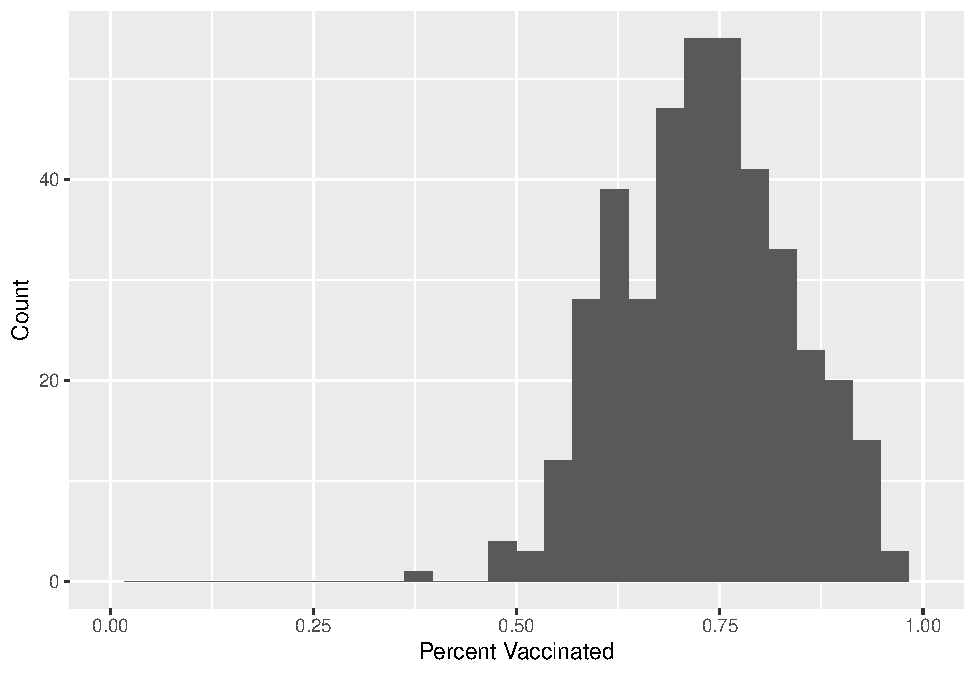
\includegraphics{COVID-19-Vax-mini-project_files/figure-latex/unnamed-chunk-34-1.pdf}

\begin{quote}
Q19. Is the 92109 and 92040 ZIP code areas above or below the average
value you calculated for all these above?
\end{quote}

\begin{Shaded}
\begin{Highlighting}[]
\NormalTok{vax }\SpecialCharTok{\%\textgreater{}\%} \FunctionTok{filter}\NormalTok{(as\_of\_date }\SpecialCharTok{==} \StringTok{"2022{-}03{-}01"}\NormalTok{) }\SpecialCharTok{\%\textgreater{}\%}  
  \FunctionTok{filter}\NormalTok{(zip\_code\_tabulation\_area}\SpecialCharTok{==}\StringTok{"92040"}\NormalTok{) }\SpecialCharTok{\%\textgreater{}\%}
  \FunctionTok{select}\NormalTok{(percent\_of\_population\_fully\_vaccinated)}
\end{Highlighting}
\end{Shaded}

\begin{verbatim}
##   percent_of_population_fully_vaccinated
## 1                               0.551981
\end{verbatim}

\begin{Shaded}
\begin{Highlighting}[]
\NormalTok{vax }\SpecialCharTok{\%\textgreater{}\%} \FunctionTok{filter}\NormalTok{(as\_of\_date }\SpecialCharTok{==} \StringTok{"2022{-}03{-}01"}\NormalTok{) }\SpecialCharTok{\%\textgreater{}\%}  
  \FunctionTok{filter}\NormalTok{(zip\_code\_tabulation\_area}\SpecialCharTok{==}\StringTok{"92109"}\NormalTok{) }\SpecialCharTok{\%\textgreater{}\%}
  \FunctionTok{select}\NormalTok{(percent\_of\_population\_fully\_vaccinated)}
\end{Highlighting}
\end{Shaded}

\begin{verbatim}
##   percent_of_population_fully_vaccinated
## 1                               0.723778
\end{verbatim}

Both values are below the mean we found above. 0.754\textgreater0.724
0.754\textgreater0.552

\begin{quote}
Q20. Finally make a time course plot of vaccination progress for all
areas in the full dataset with a age5\_plus\_population \textgreater{}
36144.
\end{quote}

\begin{Shaded}
\begin{Highlighting}[]
\NormalTok{vax.}\FloatTok{36.}\NormalTok{all }\OtherTok{\textless{}{-}} \FunctionTok{filter}\NormalTok{(vax, age5\_plus\_population }\SpecialCharTok{\textgreater{}} \DecValTok{36144}\NormalTok{)}

\FunctionTok{ggplot}\NormalTok{(vax.}\FloatTok{36.}\NormalTok{all) }\SpecialCharTok{+}
  \FunctionTok{aes}\NormalTok{(as\_of\_date,}
\NormalTok{      percent\_of\_population\_fully\_vaccinated, }
      \AttributeTok{group=}\NormalTok{zip\_code\_tabulation\_area) }\SpecialCharTok{+}
  \FunctionTok{geom\_line}\NormalTok{(}\AttributeTok{alpha=}\FloatTok{0.2}\NormalTok{, }\AttributeTok{color=} \StringTok{"blue"}\NormalTok{) }\SpecialCharTok{+}
  \FunctionTok{ylim}\NormalTok{(}\FunctionTok{c}\NormalTok{(}\DecValTok{0}\NormalTok{,}\DecValTok{1}\NormalTok{)) }\SpecialCharTok{+}
  \FunctionTok{labs}\NormalTok{(}\AttributeTok{x=}\StringTok{"Date"}\NormalTok{, }\AttributeTok{y=}\StringTok{"Percent Vaccianted"}\NormalTok{,}
       \AttributeTok{title=}\StringTok{"Vaccination rates across California"}\NormalTok{,}
       \AttributeTok{subtitle=}\StringTok{"only areas with a population above 36k are shown"}\NormalTok{) }\SpecialCharTok{+}
  \FunctionTok{geom\_hline}\NormalTok{(}\AttributeTok{yintercept =}\NormalTok{ ave}\FloatTok{.36}\NormalTok{, }\AttributeTok{linetype=}\StringTok{"dashed"}\NormalTok{)}
\end{Highlighting}
\end{Shaded}

\begin{verbatim}
## Warning: Removed 311 row(s) containing missing values (geom_path).
\end{verbatim}

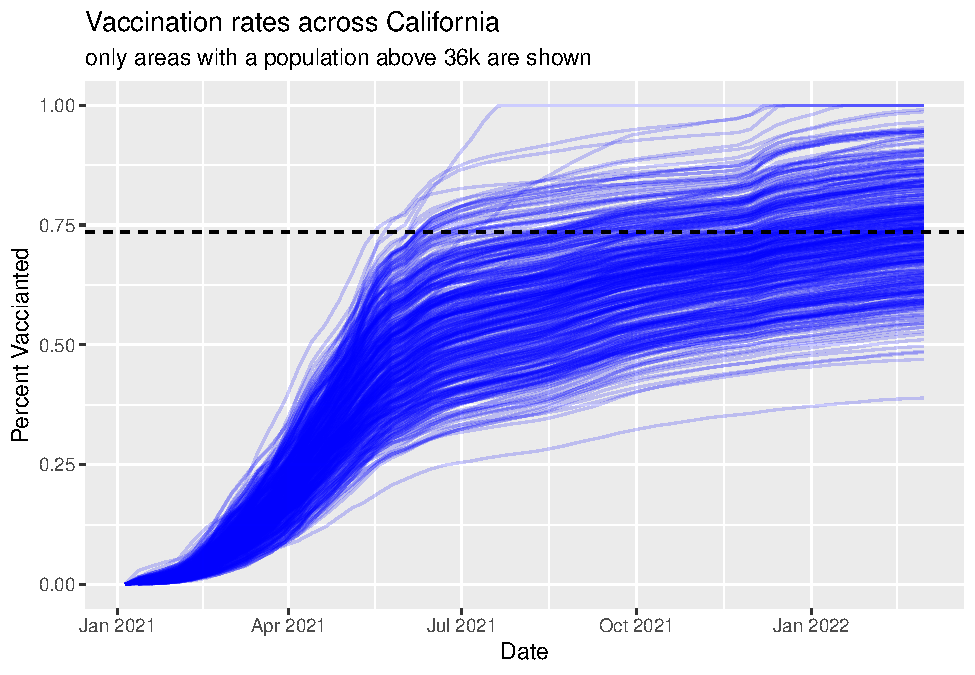
\includegraphics{COVID-19-Vax-mini-project_files/figure-latex/unnamed-chunk-37-1.pdf}

\begin{quote}
Q21. How do you feel about traveling for Spring Break and meeting for
in-person class afterwards?
\end{quote}

I grduate this quarter so while I would be down to travel, I won't be a
student anymore next quarter :(

\end{document}
